% !TEX root = ../main.tex

\chapter{Probabilistic Programming -- the User's Perspective}
\label{chp:probprog}

Probabilistic programming systems (PPSs) allow users to define probabilistic models 
using a domain-specific programming language or modeling library. A probabilistic program implicitly 
defines a distribution on random variables, whilst the system back-end implements 
general-purpose inference methods.  Two key challenges for a PPS are in providing the
syntax and semantics to allow easy definition of models, and in designing the solvers, i.e.
inference engines, to provide effective inference for those models.
In this chapter, we focus on the former of these, providing an introduction to 
probabilistic programming from a user's perspective, explaining how it can be used for, and
to extend, conventional Bayesian modeling and how it can also be used to reinterpret many computational simulation
techniques not usually associated with Bayesian modeling in a more Bayesian mindset.
We will mostly ignore the rather major issue of how to construct automated inference engines for probabilistic
programs, returning to address this in Chapter~\ref{chp:proginf}.
Here we will explain how general purpose PPSs aim to  provide 
the \emph{flexibility} to define
wide ranging and potentially obscure models, the \emph{expressivity} of a framework for 
model definition that is more in line we conventional scientific simulation than mainstream 
statistical approaches, and the \emph{automation} to  run any problem the user might write
by decoupling model specification and inference.
Together these characteristics produce a framework that allows researchers whose expertise 
lies elsewhere, to carry out powerful statistical analyses for their application specific tasks.  
This framework also aids in the development of both inference
algorithms and models for those within the machine learning and statistics communities,
by removing many of the complications of one while developing the other.
%
%We will for now focus on a user's perspective, introducing how and why one might want to use
%probabilistic programming, explain how ideas from more mainstream Bayesian
%modeling can be transferred, and demonstrate how probabilistic programming can be
%used to both extend the traditional Bayesian framework and reinterpret many computational simulation
%techniques not usually associated with Bayesian modeling in a more Bayesian mindset.
%We will mostly ignore the rather major issue of how to conduct Bayesian inference for
%models defined in probabilistic programs, assuming for now that we have a magical
%general purpose inference engine that will solve any model we provide,
%before returning to actually confront this major stumbling
%block in Chapter~\ref{chp:proginf} once we have introduced the problems of Bayesian
%inference more generally.  We will provide a brief introduction to the Anglican PPS
%to give us a platform for providing examples and highlighting
%key components of designing a PPS.  Finally, we discuss some of the current limitations
%and opportunities for PPSs (other than the obvious computational
%issues which we return to later), in particular demonstrating how we can use them to go beyond
%standard inference frameworks and why we would want to do so.

We note that it will be necessary at times during this chapter to refer briefly to some Bayesian inference
algorithms that will not be properly introduced until Chapters\ref{chp:inf} and~\ref{chp:part}.  
We have situated this chapter before those partly in order to emphasize the point that one should not 
need an intricate knowledge of inference methods to \emph{use} PPSs.  Though it is difficult
to introduce PPSs while completely omitting reference to inference methods, readers who
are not familiar with inference methods should be able to safely ignore which methods are referred to
at a first pass, noting only that different inference algorithms have different requirements and sets 
of problems they perform well on, and thus that the design of a PPS is intricately linked to the inference
method(s) used.

% !TEX root = ../main.tex

\section{Inverting Simulators}
\label{sec:probprog:inv}

Though the use of Bayesian modeling through the sciences and engineering is widespread,
it is still dwarfed by the use of simulators more generally.  Some simulations are inherently
probabilistic, such as many of those used in statistical physics~\citep{landau2014guide},
 financial modeling~\citep{jackel2002monte}, and weather prediction~\citep{evensen1994sequential}.  
 Others are deterministic approximations
of a truly stochastic world, such as lap time simulation for formula one cars~\citep{perantoni2014optimal}
and finite element simulations for fluid dynamics~\citep{versteeg2007introduction}.
In many of these scenarios, real data is also available, but not in sufficient quantities that the carefully
constructed simulations can be done away with entirely and replaced by a purely data driven
approach.  
Imagine the potential utility of general purpose methods for incorporating real data
into these simulators to improve them, without having to throw away the existing carefully constructed models.  
What about if we could even find methods for automatically
inverting these simulators?  Given a target lap time, we could return the best car setup; given observations
of, and a simulator for, human behavior, we could learn about the underlying cognitive processes; given
a climate change model and measurements, we might infer what the driving factors are.  

An ambitious long
term aim of probabilistic programming is to solve such problems and to do so in an automated fashion
so that it requires little or no statistical expertise on the behalf of the user, allowing for simple, widespread usage
across many fields.  The key realization is that stochastic simulators implicitly define probability distributions.
They, therefore, represent generative models and using probabilistic programming we can reason about, and
work with, these generative models explicitly.  One typically thinks of Bayesian modeling in terms of the
prior and the posterior, but one can also think about it in terms of defining a joint distribution over
both parameters and data, then fixing the latter to the actual observations to get a conditional distribution from
this joint.  Simulators implicitly define such joint distributions, with the outputs of the simulator corresponding
to the data, and the inputs and internal variables the parameters.  Probabilistic programming allows us to turn this on its head,
using the same code as the original simulator, but instead providing the observed data as the input and
then inverting the simulator through inference to learn about possible input parameters and other 
variables sampled during the program's forward execution.  
As well as the clear direct utility of allowing such inversion, this process also allows us to improve
our simulator using real data, by calculating the posterior predictive distribution that incorporates both
the original model and the information from the data.

To explain what we mean by inverting simulators more precisely, we will now consider
the example of inferring Captchas~\citep{mansinghka2013approximate}.   Even if the name is not familiar, 
everyone should hopefully have come across Captchas before when a website shows us an image, such
as those in in Figure~\ref{fig:probprog:example_captchas}, and asks us to
type the characters in that image to demonstrate we are not a robot.  We now ask the
question: how might we write an algorithm that breaks this Captcha by 
automatically predicting these characters directly from the image? In other words, 
can we build a robot that mimics a human on a task specifically designed to 
distinguish between the two.  If we had access to large supply of training examples, i.e.
character-image pairs, we could of course use an off-the-shelf discriminative algorithm:
neural networks have been used to try and solve the problem in exactly this way with reasonable
success~\citep{von2008recaptcha}.  However, without access to an abundance of data this is a rather
challenging task and we will need to exploit our prior knowledge about the problem.  

\begin{figure}[t]
	\centering 
	\begin{subfigure}[t]{0.58\textwidth}
		\centering
			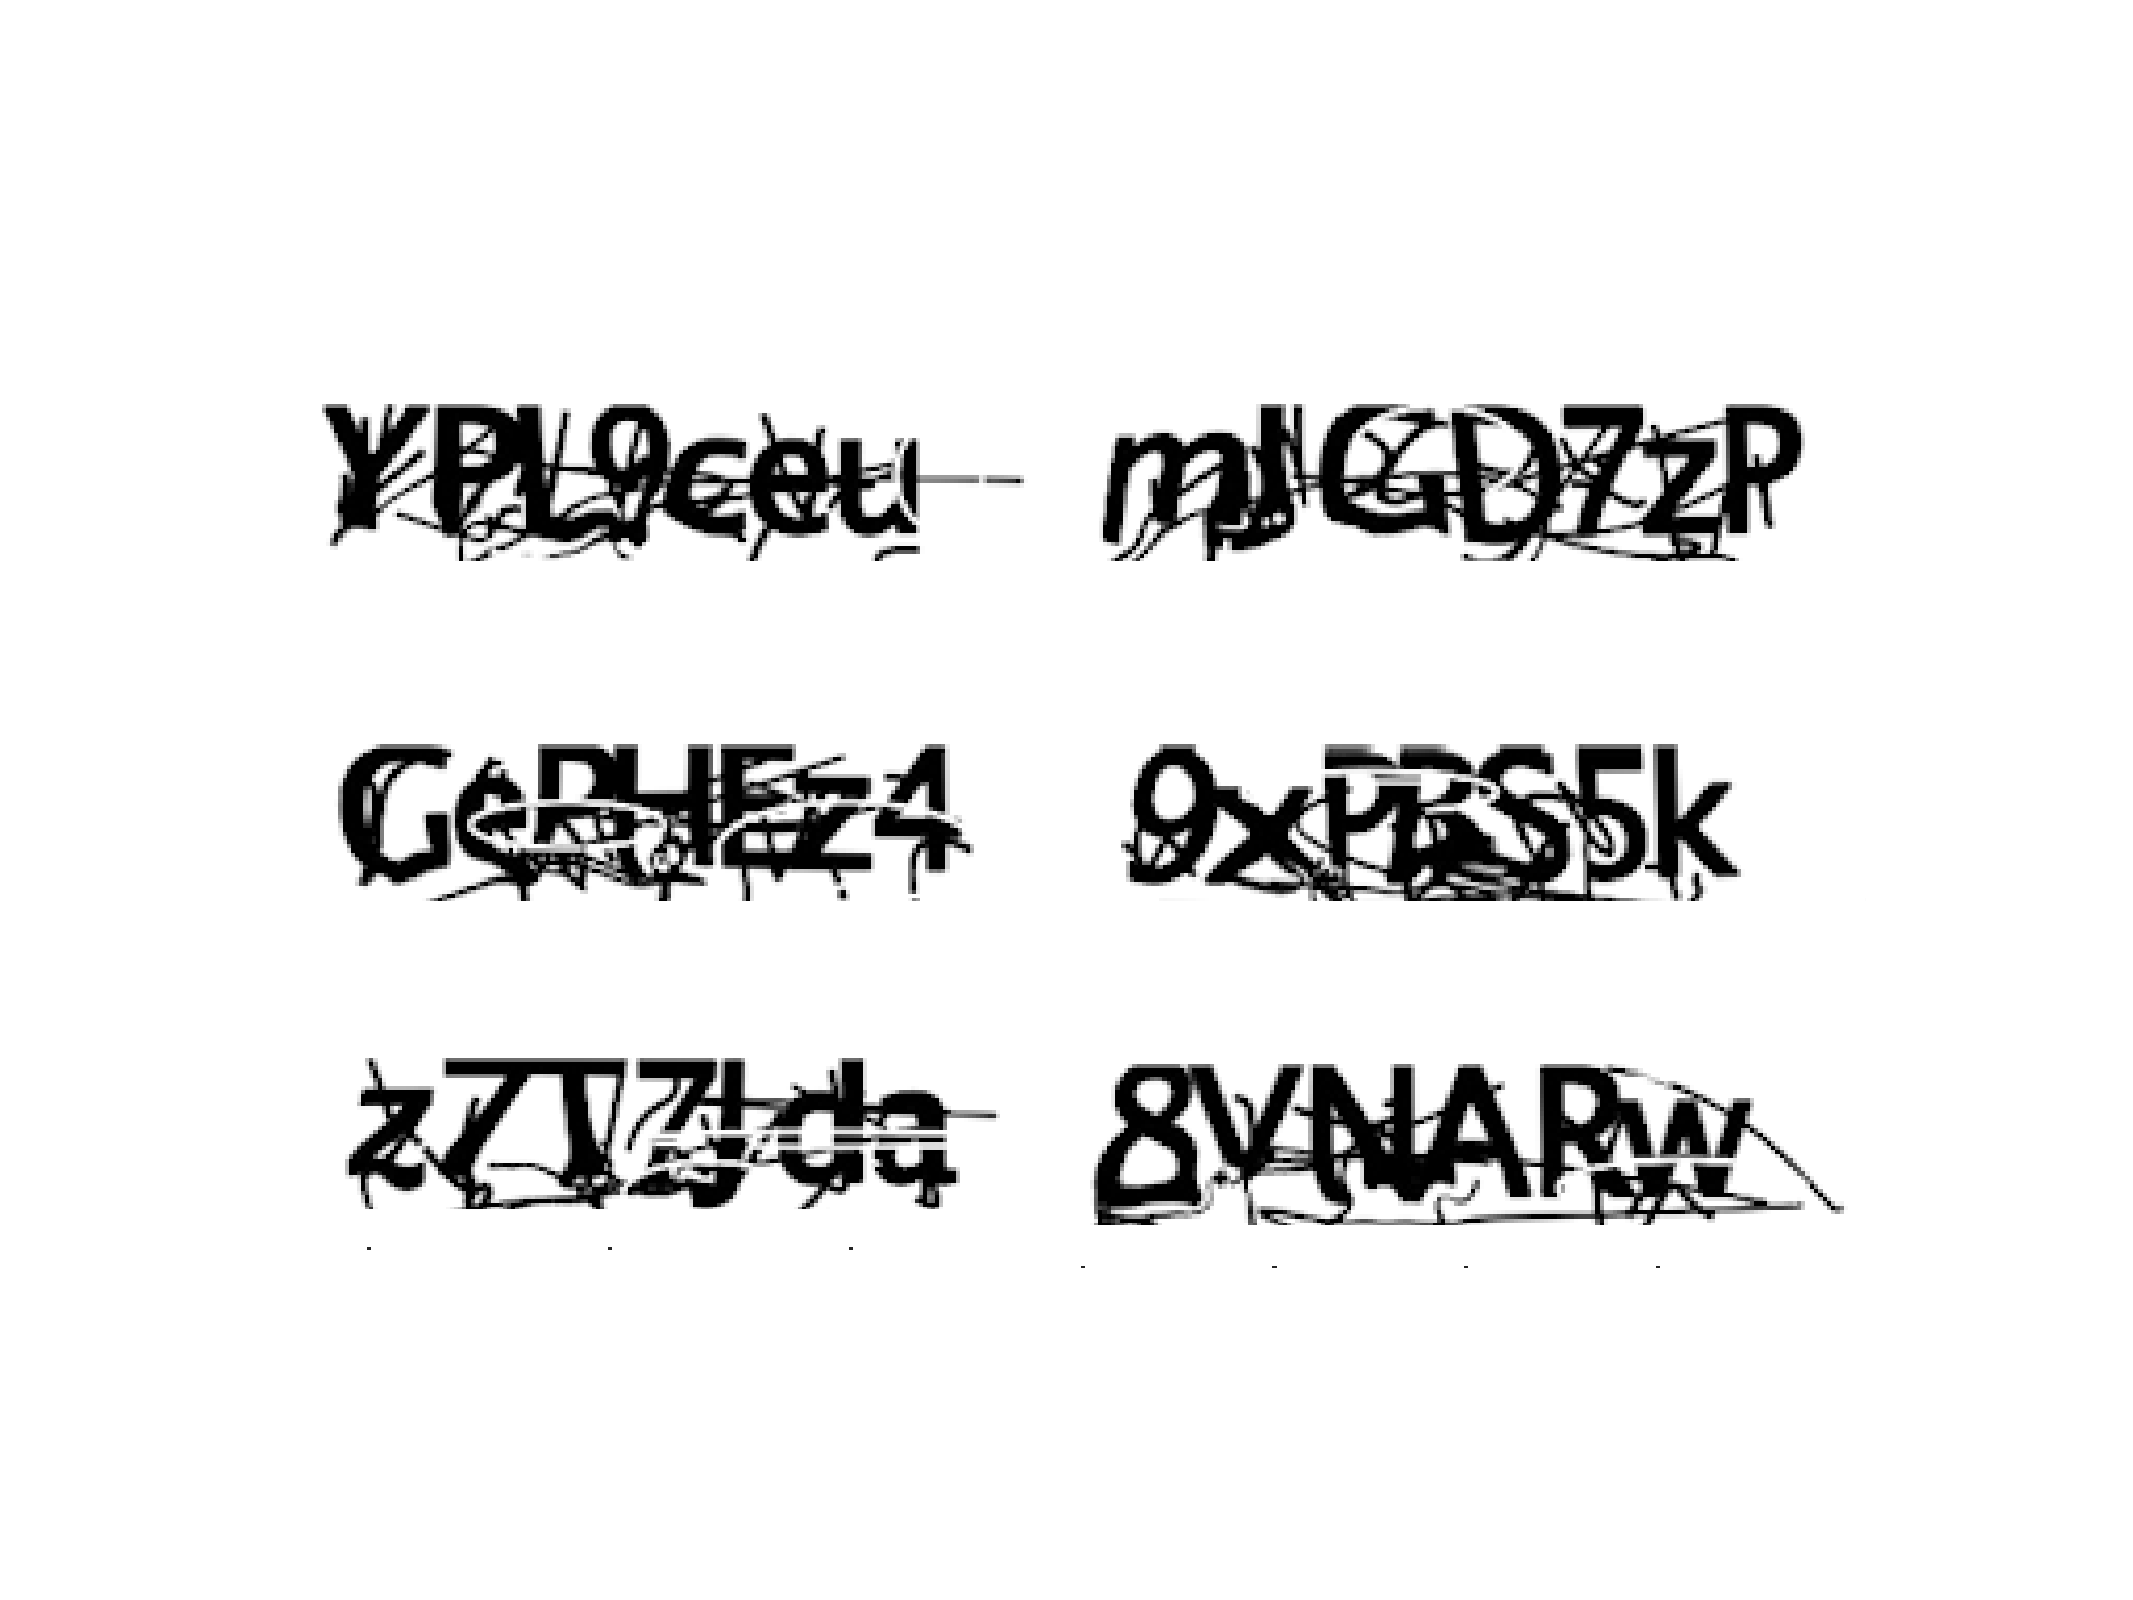
\includegraphics[width=\textwidth]{probprog/figures/example_captchas.pdf}
		\caption{Examples of real Captchas
			 \label{fig:probprog:example_captchas}}
	\end{subfigure}
	~~
	\begin{subfigure}[t]{0.38\textwidth}
		\centering
			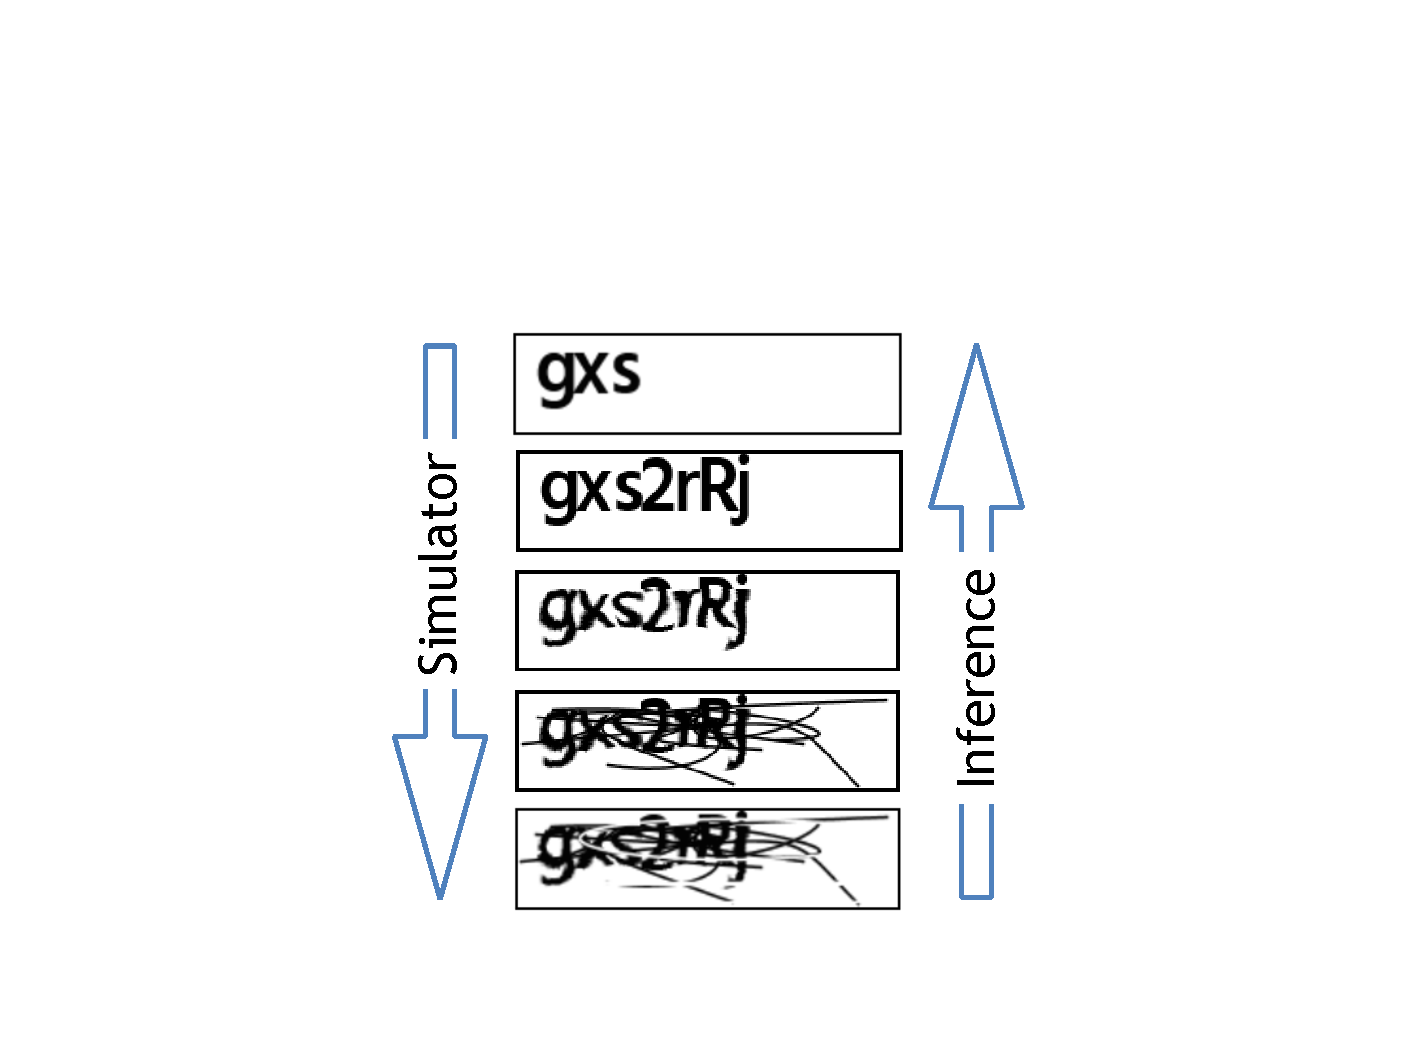
\includegraphics[width=\textwidth]{probprog/figures/captcha_sim.pdf}
		\caption{Example simulation of a Captcha
			\label{fig:probprog:captcha_sim}}
	\end{subfigure}
	\vspace{5pt}
	\caption{Solving Captchas by simulator inversion.   \textbf{(a)} gives examples of real
		Facebook Captchas taken from~\cite{le2017using}.  Here the corresponding
		generating strings going
		to clockwise from the top left are YPL9ceu, mJGD7zP, 9xPBS5k, 8VNARw, z7T7Jda, and
		GePHEz4.  A user is asked to type in these strings when shown the corresponding
		image to show they are not a robot.
		\textbf{(b)} gives an example of the process of simulating Captchas taken by
		~\cite{le2017inference}.  Here we see that we can generate a Captcha by first
		simulating a series of characters, then simulating appropriate manipulations 
		to those characters such as warping, rotating, and adding noise.  Inverting this
		simulation process corresponds to an inference problem, where we want to find
		out the characters that lead to a particular image.
		\label{fig:probprog:captcha}}
\end{figure}

Doing this process in reverse, i.e. simulating a Captcha, on the other hand, is a substantially
less daunting process.  The true Captchas are actually generated by
a simulator and so we can attempt to mimic this original simulation process.
For example, as shown in Figure~\ref{fig:probprog:captcha_sim} we might first sample a 
number of characters, then a symbol for each character, apply manipulations such as rotations and warpings, simulate
some obscuring lines or other noise, and finally render our simulated components into an
image.  Though admittedly it might take some time and effort to construct a high fidelity
simulator that well matches the produced images, the technical requirements for doing this
(other than possibly the final rendering) are minimal and so it could be carried out by most
people with a reasonable degree of experience in scientific programming.  The number of
people able to write such a simulator should certainly be substantially larger than the
number of people with sufficient experience in Bayesian modeling to construct an equivalent
graphical model or direct mathematical formulation.  The number of people
with the expertise to then write an appropriate inference scheme for the problem is even
smaller.  In a PPS, writing this simulator and providing the data is all that is required.
Given these, the PPS will carry out the inference required to invert the simulator automatically,
inferring the characters from the image.  More generally, we are estimating the inputs and
internal variables of our simulator, given target values for the outputs.

There are two key factors to realizing our aim of inverting simulators.  Firstly we need to provide a 
language which easily allows users to
write down simulators and which has semantics that allows the compiler to extract an appropriate
representation of the joint distribution.  In other words, we need our language to be sufficiently
general purpose and easy to use to not burden the user, while at the same time having syntax and semantics that
ensure the corresponding joint distribution is well defined and can be converted into a form where
we can run inference.  Doing this will require the introduction of means for \emph{conditioning} on data
and of specially defined \emph{random primitives} whose behavior can be controlled at 
run time, rather than just always sampling from
the same predefined distribution as they would in an ordinary programming language.  
The latter can be thought of as defining terms in the prior and the
former as terms in the likelihood as we will discuss in Section~\ref{sec:probprog:models}.
For certain cases, one can alternatively think of conditioning as applying \emph{constraints} to the
program.  For example, we can think of a probabilistic program as defining a simulator
and a set constraints that must be satisfied; this is exactly
how the PPS Church~\citep{goodman2008church} is designed.  An important distinction 
here though is between \emph{hard} and \emph{soft} conditioning.  Hard conditioning is as per the conventional
interpretation of a constraint -- we condition on the fact that an event occurs exactly.  Soft conditioning instead
assigns a weight to the program based on the probability (or probability density) of a given event occurring.
Though hard conditioning is a particular case of soft conditioning (for which the weight is either 1 or 0),
one can, at least semantically, use it to specify a soft conditioning, say 
$p(Y=y | X=x)$, by sampling $Y\sim p(y|X=x)$ and then imposing the constraint $Y=y$.
However, only supporting hard conditioning in a PPS is somewhat restrictive for practical
use, as one cannot effectively condition on continuous data because there is zero probability of
satisfying the resulting constraint.

The second key factor is that our language needs a general purpose inference(s)
engine capable of working on any program the user writes.  Bayesian models are fully defined
by their joint distribution and the data.  Therefore, once a user has written their simulator and provided
the data, this uniquely defines a posterior and the only problem is in solving the resulting Bayesian inference.
If we can now construct inference engines capable of working on arbitrary code, we can 
automate inference on any simulator or model the user defines, creating an
abstraction barrier between model definition and drawing inferences from that model.  We will discuss how this can be
done at length in Chapter~\ref{chp:proginf}.

If we can construct a system that can successfully carry out these tasks, 
the huge potential applications this could provide should be clear. We would have a 
system where the user requires no expertise in inference or conventional
Bayesian modeling in order to write application specific models and have them solved automatically.
Instead, they need only have the ability to write stochastic simulators for the process they wish to
model, a skill possessed my most of the scientific community and many of those outside it as well.
In a hypothetical future where scientists
code all their simulators in extremely powerful PPSs, tasks such as
inverting those simulators and improving the simulator by incorporating real data would
be automated in the same way current compilers convert high-level coding languages to machine code.  
However, this ability is not completely
hypothetical -- many such problems can already be handled by existing systems.  The challenge
is improving and scaling such systems to deal effectively with more difficult and more wide ranging models
in a tractable manner.  The need for such systems to work in an automated manner for a wide array
of possible problems makes this a very difficult problem; after all we are somewhat flaunting the no-free-lunch
theorem.  However, there is a key component that provides hope that this may be possible: we have access
to the target source code of the simulator itself, rather than needing to treat it as a black-box as is the
case for, say, approximate Bayesian computation (ABC) methods~\citep{csillery2010approximate}.  Therefore
maybe we can have our cake and eat it by using the source code itself to guide our algorithms, such that
they behave in problem specific ways.  We will discuss how this can be done at length in 
Chapters~\ref{chp:proginf} and~\ref{chp:bopp}.
% !TEX root = ../main.tex

\section{Differing Approaches}
\label{sec:probprog:two}

Rather than being a clearly defined method,
probabilistic programming is more of an umbrella term that covers a spectrum of 
different approaches, varying from inference toolboxes through to universal probabilistic programming
languages (PPLs) that allow
arbitrary probabilistic code to be written.
%, even that which might not correspond to a valid model.  
Often there is a trade-off between efficiency and expressivity: the more restricted
one makes the language, the more those restrictions can be exploited to improve the efficiency
of the inference.  This leads itself two distinct philosophies when developing a system. 
Firstly one can start with a particular inference algorithm and then design a system around making it as
easy as possible to write models for which that inference algorithm is suitable.  Secondly one can start
with  a general purpose PPL that allows as many model as possible to be written and then try to construct
inference engines that are capable of work in such a general framework.  Both approaches 
have their merits and drawbacks, with the distinction typically coming down to the intended use.
We will now elucidate each approach more precisely.  

\subsection{Inference Driven Systems}
\label{sec:probprog:two:inf}

Though there is a plethora of bespoke inference algorithms designed for particular models, the vast majority of these are based around
a relatively small number of foundational methods such as importance sampling, sequential Monte Carlo,
Metropolis-Hastings, Gibbs sampling, message passing, and variational inference (see Chapter~\ref{chp:inf}).
The extensive use of these core inference approaches throughout Bayesian statistics and machine
learning means that it makes clear sense to write packages for automating them and which
make it easy for the user to define an appropriate graphical models for which the inference can be automated.
This both improves efficiency of modeling and reduces barriers to effective Bayesian modeling by reducing the
required inference expertise for users.  This inference-first philosophy is taken by a number of successful PPSs
and inference toolboxes (the distinguishing line between which can be a little blurry), a small number of which we now 
briefly outline.

BUGS (Bayesian inference Using Gibbs Sampling) \citep{spiegelhalter1996bugs} and its 
	extensions~\citep{lunn2000winbugs,plummer2003jags,todeschini2014biips}
	allow finite DAGs to be specified using declarative code or pictorially using a graphical user
	interface.  These are converted to a form that is suitable for inference, the exact nature of which
	depends on the implementation, with the original work being based on Gibbs sampling.
	
Infer.Net \citep{minka_software_2010} is modeling language for defining, and automating approximate inference in
	both DAGs and Markov random fields, using predominantly message-passing algorithms. Distributions
	are generally, though not exclusively, restricted to be exponential families.  Branching (i.e. \texttt{if}) 
	is allowed, but requires enumeration of all possible paths at run time.

LibBi \citep{murray2013bayesian} is a package for doing Bayesian inference for state-space models,
	using particle-based inference methods (see Chapter~\ref{chp:part}).  It has a strong focus on scalable
	computation, providing support for multi-core architectures and graphics processing units.

PyMC3 \citep{salvatier2016probabilistic} is a python framework for carrying out MCMC and variational
	inference, using Theano~\citep{bergstra2010theano} to calculate the gradients required by some inference methods.

Stan \citep{carpenter2015stan} is a PPS with interfaces to many difference languages and a
	focus on performing Hamiltonian Monte Carlo inference~\citep{duane1987hybrid,hoffman2014no}, though
	other inference methods such as variational inference are also provided~\citep{kucukelbir2015automatic}.
	As with PyMC3, automatic differentiation is used to calculate required gradients.  The need to take
	derivatives means that there is limited support for discrete variables or branching.

These systems do not allow users to write models that would be difficult (at least for
an expert) to code without a PPS -- in general they all can be thought of as defining a graphical model
or sometimes factor graph -- but they offer substantial utility through ease of model exposition and
automating inference.

\subsection{Universal Probabilistic Programming}
\label{sec:probprog:two:general}

As useful as these inference-driven systems are, they do not fit very well with the notion of
inverting simulators we introduced in Section~\ref{sec:probprog:inv}.  They are still closely tied
to graphical models and are more toolboxes for streamlining the Bayesian modeling process than
a means of writing models that would be problematic to define by conventional means.  Achieving
our long term ambitious aim of making general purpose systems for conducting inference of
arbitrary simulators will require us to take a somewhat different approach that instead starts
with a general-purpose language and then attempts to design inference algorithms capable of
working on arbitrary models and code.  It will be necessary for such systems to
support models where the set of random variables is dynamically typed, such that it is possible 
to write programs in which this set, and thus potentially the number of random variables, differs 
from execution to execution.  To avoid hindering the user or restricting the models which can be
defined, it will important to allow 
things such as branching, recursion, higher-order functions,
conditional existence of variables, and arbitrary black-box
deterministic functions.  Ideally, we would like to provide no restrictions on the code that the user
can write, except for eliminating programs do not define valid probability distributions, such as
those that have a non-zero probability of never terminating.  In practice catching such invalid cases can
be hard or even impossible and so many systems actually adopt a philosophy of applying no restrictions,
such that it is perfectly possible to define invalid models.  General purpose PPSs actually bring up new
theoretical questions about what constitutes a valid probability model~\citep{heunen2017convenient}, while
even the set of valid definable models is a strict super-set of the those definable by graphical models 
for many systems~\citep{goodman2013principles}.

In the rest of this thesis, we will predominantly focus on these \emph{universal} PPLs~\citep{goodman_uai_2008,staton2016semantics}, 
so-called because they are based on \emph{Turing complete} languages that can specify any
computable distribution~\citep{goodman2013principles}.  For our purposes, we further refine this definition
to systems that also allow specification for any computable conditioning.
We will regularly using the universal PPL Anglican~\citep{wood2014new} as a reference, an introduction
to which is provided in Section~\ref{sec:probprog:anglican}. Here we will briefly discuss some other
prominent higher order PPLs.

Church is a PPL based on Scheme \citep{goodman_uai_2008}.  
The original seminal paper and accompanying system 
	forms a foundation on which many of the prominent existing systems are built through its
	demonstration that higher-order probabilistic programs define valid probability models, even in
	the presence of infinite recursion.  However, Church predominantly only allows hard
		conditioning,\footnote{Some very limited support for soft-conditioning is provided in current
		implementations through a ``noisy equals'' that equates to a Gaussian likelihood.}
	namely a model in Church comprises of a generative sampler and a separate predicate procedure
	which returns true if the desired conditions are satisfied.  
	In addition to the aforementioned issues of hard conditioning, this complete separation of the 
	generative process and the conditioning can also be wasteful in not allowing the structure of a 
	model to be exploited (see Chapters~\ref{chp:part} and \ref{chp:proginf}).  
	Later systems therefore mostly allow soft conditioning statements to be interleaved
	through the generative progress (in an analogous manner to likelihood terms), increasing the range
	of (solvable) models than can be encoded and the potential efficiency of inference algorithms.
	Inference in Church (and its direct derivatives) is typically carried out using either rejection sampling
	or MCMC.  Church places a particularly strong emphasis on the ability to carry out \emph{nested inference},
	something we will look into in depth in Chapter~\ref{chp:nest}.

Venture~\citep{mansinghka2014venture} is a probabilistic programming platform providing a flexible
system for both specification of models and inference methods.  In has a strong emphasis on being extensible
and for allowing the hosting of eternal applications.  For example, it allows the user to provide proposals for
the inference engine or reprogram the inference strategy entirely.  Venture is predominantly used via the
VentureScript~\citep{mansinghka2014venture} PPL.

WebPPL \citep{goodman_book_2014} is a PPL built using a purely functional subset of Javascript,
conveniently allowing for embedding in web pages.
In combines the ability to write a generative process using sampling statements and to add in likelihood
terms through a {\small \texttt{factor}} primitive that is analogous to the \observe primitive that we will introduce
in Section~\ref{sec:probprog:models:first}.  At its back end, WebPPL provides a number of different inference
algorithms, such as SMC and MCMC methods.

The price for the expressivity of these general purpose systems is a substantial extra 
burden on the inference engine as we will
discuss in Chapter~\ref{chp:proginf}.  In general, inference methods for such systems 
must be formulated in such a manner that they are applicable to models where the 
density function is intractable and can only be evaluated during forwards simulation of the program. 
For example, it may not be possible to know if a variable is continuous or discrete except by
running the program, while some variables will only exist conditioned on the values of others.
This required generality of the inference engine will naturally lead to a drop in performance compared to
custom written inference code, but this is often a price worth paying for generality and automation, particularly
when considering models that would be challenging to express, let alone do inference in, using more
conventional frameworks.
% !TEX root = ../main.tex

\section{Bayesian Models as Program Code}
\label{sec:probprog:models}

In the last section we shown how we can thing of PPS as inverting simulators, predicting internal
variables and the inputs given the outputs.  In this section we will take a different perspective and
show how we can translate Bayesian modeling into the framework of program code.  As we 
showed in Chapter~\ref{chp:bayes} we showed how a Bayesian model is defined by a prior over
parameters and a likelihood function for those parameters given the data.  This viewpoint will
mostly translate into the probabilistic programming setting by equating between the prior
and sampling statements and between the likelihood and conditioning statements.  At the end
of the section we will explain why this is actually a slight approximation (in short because we
might condition on internally sampled variables) but for most purposes this viewpoint will suffice.
We will keep things predominantly high-level for now, giving a more detailed look in
Section~\ref{sec:probprog:anglican} by introducing a particular PPS, namely Anglican, in detail.

\subsection{A Simplified Probabilistic Programming Setup}
\label{sec:probprog:models:first}

We start by considering the case of constructing a restricted PPS.  We will presume that our
language has no branching (i.e. no \texttt{if} statements or equivalent), is  first order
(i.e. variables cannot be functions), that there is no recursion, and that it does not allow 
any conditioning on internally sampled variables.  
We will give our language
two special constructs, \sample and \observe, between which the distribution of the
program is defined.  As such the program should not include any other random components.
Informally, \sample will be used to specify terms in the prior and \observe terms in the
likelihood.  More precisely, \sample will be used to make random draws $x_t \sim f_t(x_t | \Xi_t)$,
where $\Xi_t$ is a subset the other variables in scope at the point of sampling, and \observe will use to condition on
data $g_s(y_s|\Lambda_s)$ with $\Lambda_s$ defined in the same way as $\Xi_t$.  We presume that the program takes 
in as input external parameters $\theta$ and data $y_{1:S}$, the former of which is taken as inputs that are 
not ``observed'' at any point but can effect the conditioning through $\Xi_t$ and $\Lambda_s$, while we presume 
for our simplified setup that the latter appears in neither $\Xi_t$ or $\Lambda_s$.
We define both \sample and \observe as adding a factor to the joint distribution which is therefore given by
\begin{align}
\label{eq:probprog:simple-joint}
p(x_{1:T},y_{1:S} | \theta) = \prod_{t=1}^{T} f_t(x_t | \Xi_t) \prod_{s=1}^{S} g_s(y_s|\Lambda_s).
\end{align}
The two vary in whether they define a new random variable or effect the probability of the
program given particular instances of the other random variables.
Our presumptions for this simplified setup that no $y_{s}$ terms are present in the $\Xi_t$ or $\Lambda_s$
and that we do not condition on internally sampled variables, means that we can here have
exactly that our prior is $\prod_{t=1}^{T} g_t(x_t | \Xi_t) =: p(x_{1:T} | \theta)$ and our likelihood is
$\prod_{s=1}^{S} g_s(y_s|\Lambda_s) =: p(y_{1:S} | x_{1:T}, \theta)$.  Consequently, for our simplified setup,
each program defines a finite directed acyclic graphical model (see Section~\ref{sec:bayes:paradigm:graph})
where the conditional relationships are defined through the definitions of $f_t$ and $g_s$.
This breakdown into a prior and likelihood and the equivalence to graphical models
will not hold in the more general cases we consider later.  \todo[inline]{Some example programs and equivalent
	graphical models for our simplified setup are given in Figure INSERT}

An important point to note is that~\eqref{eq:probprog:simple-joint} shows that all of our \sample
and \observe statements are exchangeable, in the sense that their order can be moved around and
still define the same joint distribution, up to restrictions about all the required variables required
for the conditioning existing and being in scope.  For example, if all variables remain in scope
and are not redefined, we can generally move all our \observe statements to the end of the program
without changing the joint distribution.  Nonetheless, the position of the \observe statements
can often be important from the perspective of the performance of the inference engine.  This exchangeability
result will carry over to the non-simplified cases.

Other than \sample and \observe statements, the rest of our program is by construction totally deterministic.  Therefore,
though it may contain random variables other than $x_{1:T}$, these random variables are deterministic
functions of the ``raw'' random draws $x_{1:T}$ and inputs $\theta$ and $y_{1:S}$.  We can therefore 
define the outputs of our program as $z := h(x_{1:T},y_{1:S},\theta)$ for some deterministic function $h$.
As we explained in Section~\ref{sec:prob:measure}, the change of variables means that the density function on $z$,
$p(z | y_{1:S}, \theta) $
can have a different form to the posterior implied by our program, namely $p(x_{1:T} | y_{1:S}, \theta)$.
  Though this is a serious complication in the
context of optimization (we may not in general be able to find $\argmax_z p(z|y_{1:S},\theta)$
or even evaluate $p(z | y_{1:S}, \theta)$ exactly), it
is perfectly acceptable in the context of calculating expectations as
\begin{align}
\int f(z) p(z | y_{1:S}, \theta) dz = \int f(h(x_{1:T}, y_{1:S}, \theta)) p(x_{1:T} | y_{1:S}, \theta) dx_{1:T}
\end{align}
for implicitly defined measures $dz$ and $dx_{1:T}$.  Two consequences of this are that
we can express any expectations calculated by our program as expectations over $p(x_{1:T} | y_{1:S}, \theta)$
which was fully defined by the joint~\eqref{eq:probprog:simple-joint} and that, provided we are not worried
about carrying out optimizations, we do not need to explicitly worry about the implicit measures defined
by the definition of our program, other than any potential effects on the inference scheme.


%
%Because of the assumptions we have made for our language, the latent
%variables we wish to do inference for are statically determined as $x_{1:T} = x_1,\dots,x_T$ 
%such that the posterior of interest is $p_{\theta} (x_{1:T} | y_{1:S})$ (or some marginal of this for
%which we can still using Monte Carlo inference on the joint).
%
%Our implied target posterior
%is proportional to this joint in the standard way $p_{\theta}(x_{1:T}|y_{1:S}) \propto p_{\theta}(x_{1:T},y_{1:S})$.

\subsection{A General Probabilistic Programming Setup}
\label{sec:probprog:models:general}

Note that as $y_s$ terms can appear in the $\Xi_t$ terms, it can be the case that 
$p(x_{1:T} | \theta) \neq \prod_{t=1}^{T} p(x_t | \Xi_t)$ such that the latter does not
ex
can also enter \sample or \observe terms through $\Xi_t$ and $\Xi_s$ respectively.

\todo[inline]{Conditioning on internally sampled variables
	
	Ordering of decelerations matters
	
	Memoization
	
	Complications of maximization}

\section{An Introduction to Anglican}
\label{sec:probprog:anglican}

One such general purpose system, \emph{Anglican}, will be used as a reference in this paper.  In Anglican, models are defined using the inference macro \defquery. These models, which we refer to as queries \citep{goodman_uai_2008}, specify a joint distribution $p(Y,X)$ over data $Y$ and variables $X$. Inference on the model is performed using the macro \doquery, which produces a sequence of approximate samples from the conditional distribution $p(X|Y)$ and, for importance sampling based inference algorithms (e.g. sequential Monte Carlo), a marginal likelihood estimate $p(Y)$.  

Random variables in an Anglican program are specified using \sample statements, which can be thought of as terms in the prior. Conditioning is specified using \observe statements which can be thought of as likelihood terms.  Outputs of the program, taking the form of posterior samples, are indicated by the return values.  There is a finite set of \sample and \observe statements in a program source code, but the number of times each statement is called can vary between executions.  We refer the reader to  \href{http://www.robots.ox.ac.uk/~fwood/anglican/}{\small\url{http://www.robots.ox.ac.uk/~fwood/anglican/}} for more details.

\section{Going Beyond Bayesian Inference}
\label{sec:probprog:limit}

\todo[inline]{
Interpreters rather than custom languages

Avoiding bugs in code}